\documentclass[ignorenonframetext]{beamer}
\usepackage{textpos}
\usepackage{graphicx}
\usepackage{pgf}
\usepackage{listings}
\usepackage{multimedia}
\usepackage{gensymb}
\usepackage{amsmath, mathrsfs}
\usepackage{adjustbox}
\usepackage{tikz}
\usepackage{tikz-3dplot}

\usetikzlibrary{shapes.geometric, arrows.meta, calc, positioning}

\lstdefinestyle{yaml}{
     basicstyle=\ttfamily\color{blue}\tiny,
     rulecolor=\color{black},
     string=[s]{'}{'},
     stringstyle=\color{blue},
     comment=[l]{:},
     commentstyle=\color{black},
     morecomment=[l]{-}
 }

\usetheme{Boadilla}
\usefonttheme{serif}

\title[TART Position Cal]{Antenna Array Position Calibration for the Transient Array Radio Telescope}

\author[Molteno]{Tim Molteno}

\institute[Otago]
{
  Electronics Research Foundation, New Zealand \\
  \& \\
  Dept of Physics,
  University of Otago, New Zealand \\
  \& \\
  Dept of Physics \& Electronics,
  Rhodes University, South Africa \\
  \vspace{1cm}
  \vspace{2cm}
  
\includegraphics[width=0.6\linewidth]{fig/elec_header_font.pdf}
}

\logo{\pgfputat{\pgfxy(-0.72,7.7)}{\pgfbox[center,base]{
\includegraphics[width=1cm]{fig/elec_logo.pdf}}}}

\date[TART Mada 2026]{}

\begin{document}

% --- Title ---

\begin{frame}
  \titlepage
\end{frame}

% --- Introduction ---

\begin{frame}{The Transient Array Radio Telescope (TART)}
\begin{itemize}
  \item All-sky imaging interferometer operating at L1 band (1.575~GHz)
  \item Open-source project --- deployed widely for radio transient detection and imaging algorithm development
  \item 24 antennas arranged on five spiral arms
  \item Often installed during week-long workshops combining radio astronomy and hands-on telescope assembly
  \item \textbf{Key requirement:} antenna positions must be known to within $\approx 5$~mm for interferometric imaging
  \item Calibration algorithm implemented in \texttt{tart-position-cal}~\cite{moltento2026tartpositioncal}
\end{itemize}
\end{frame}

\begin{frame}{The Position Calibration Problem}
\begin{itemize}
  \item Initial positions come from nominal design --- in practice, construction deviates
  \item Must determine accurate antenna coordinates using easy-to-make measurements
  \item Must be robust to inevitable measurement errors
  \item Must fix the global rotation (distance measurements alone cannot determine orientation)
  \item Goal: accuracy to within 0.01 wavelengths at 1.575~GHz ($\approx 2$~mm)
\end{itemize}
\end{frame}

% --- Botswana calibration photo ---

\begin{frame}
 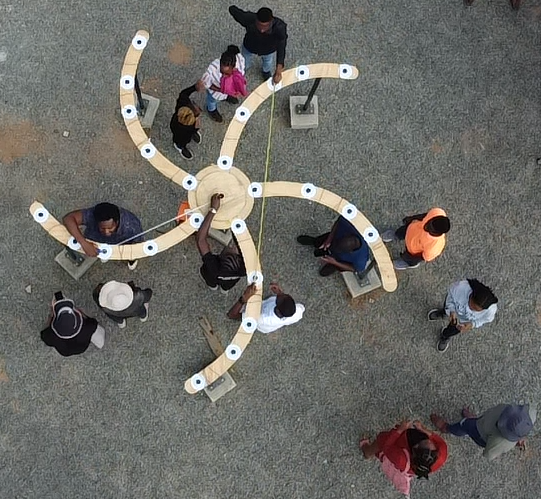
\includegraphics[width=\linewidth]{fig/botswana_calibration.png}
 \vspace{4pt}
 {\small Aerial view of a TART being calibrated by attendees at a TART workshop hosted at the Botswana International University of Science and Technology, March 2025.}
\end{frame}

% --- Method: Measurements ---

\begin{frame}{Two Kinds of Measurements}
\begin{columns}
 \begin{column}{0.55\linewidth}
  \textbf{Radial distances} $r_i$ (24 measurements):
  \begin{itemize}
    \item Distance from phase centre to each antenna centre
    \item High confidence --- single span of tape measure
  \end{itemize}
  \vspace{12pt}
  \textbf{Pairwise distances} $\delta_{ij}$ (276 measurements):
  \begin{itemize}
    \item Distance between each pair of antennas
    \item $\frac{1}{2} N (N-1)$ unique pairs for $N=24$ antennas
    \item More susceptible to measurement errors
  \end{itemize}
 \end{column}
 \begin{column}{0.45\linewidth}
  \textbf{Global rotation constraint:}
  \begin{itemize}
    \item Distance measurements are rotation-invariant
    \item Need one geographic bearing to fix absolute orientation
    \item Align one antenna arm with a distant, identifiable landmark
  \end{itemize}
 \end{column}
\end{columns}
\end{frame}

% --- Spreadsheet ---

\begin{frame}{Measurement Recording}
 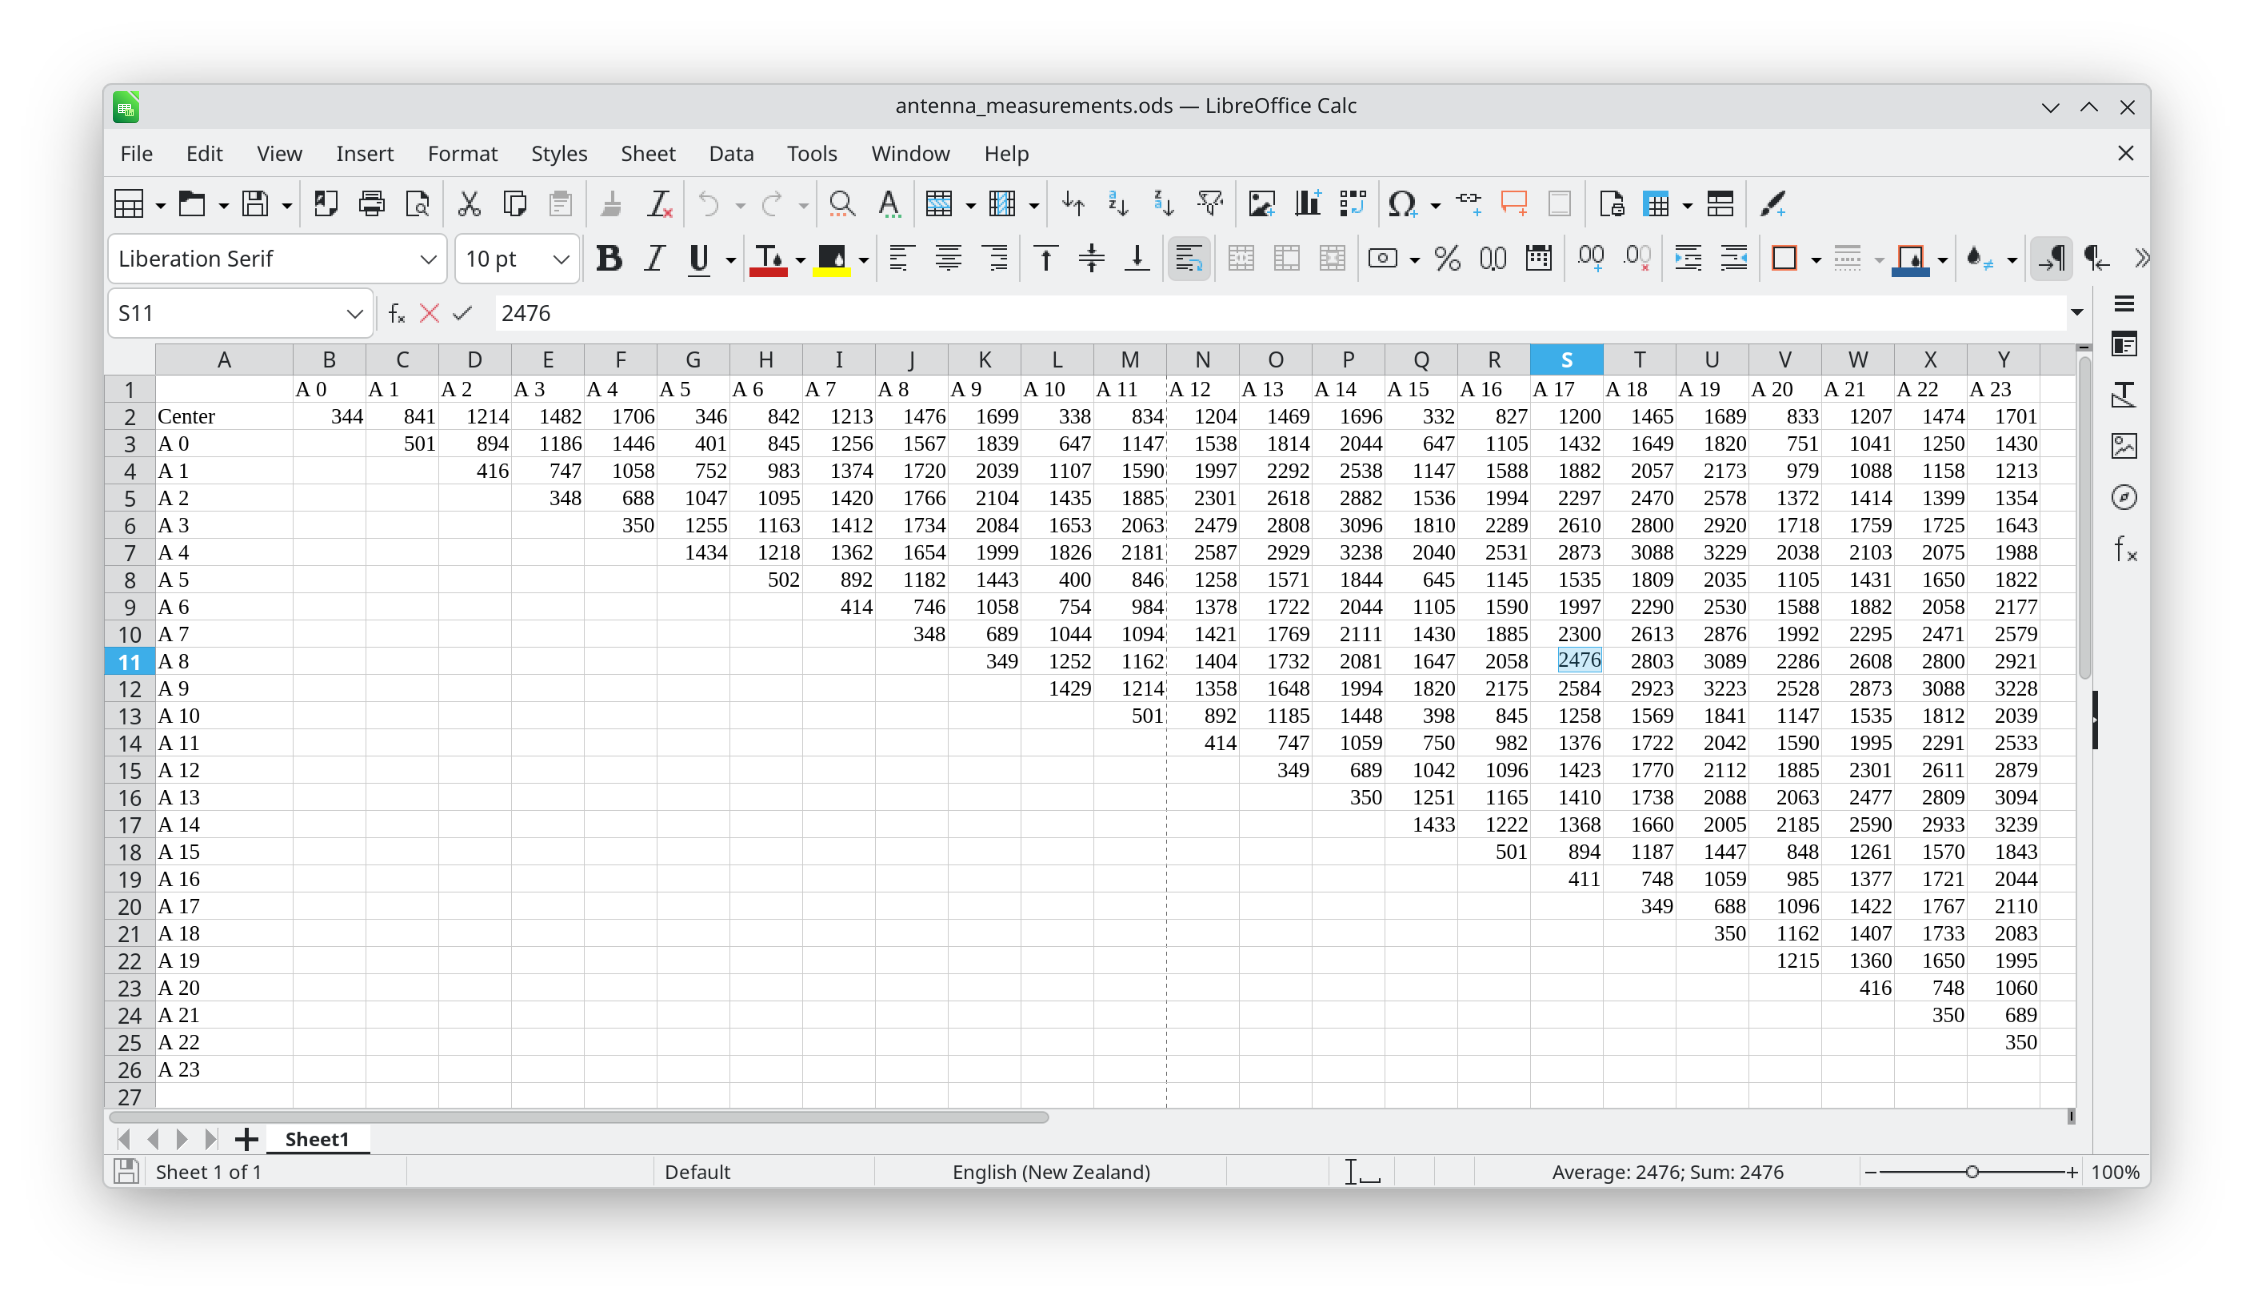
\includegraphics[width=\linewidth]{fig/spreadsheet.png}
 \vspace{4pt}
 {\small Spreadsheet with measurements from a TART array. Highlighted: distance between antenna 17 and antenna 8 (in mm).}
\end{frame}

% --- Least Squares Estimator ---

\begin{frame}{Least Squares Estimator}

Given the 24 antenna positions $\{x_i, y_i\}$ and measurements $r_i$, $\delta_{ij}$, $\theta_k$, form:

\begin{align}
 L(x, y) = w_r\, L_r(x,y) + L_{ij}(x,y) + \lambda\, L_\theta(x,y) + \gamma\, L_\chi(x,y)
\end{align}
\begin{align*}
 L_r(x,y) &= \sum_{i=1}^{N} \left( r_i - \sqrt{x_i^2 + y_i^2} \right)^2 \\[2pt]
 L_{ij}(x,y) &= \sum_{i<j} \left( \delta_{ij} - \sqrt{(x_i - x_j)^2 + (y_i - y_j)^2} \right)^2 \\[2pt]
 L_\theta(x,y) &= \left( \theta_k - \theta_k^s \right)^2
\end{align*}

\vspace{2pt}
{\small $L_r$: radial residuals. $L_{ij}$: pairwise residuals ($i<j$, 276 unique pairs). $L_\theta$: rotation constraint. $L_\chi$: chirality (reflection) constraint --- see \emph{Symmetries}, below. $w_r=10$ up-weights the more reliable radial measurements, $\lambda\approx100$ enforces rotation, $\gamma\approx10^6$ enforces chirality.}
\end{frame}

% --- Global Orientation Calibration ---

\begin{frame}{Global Orientation Calibration}
  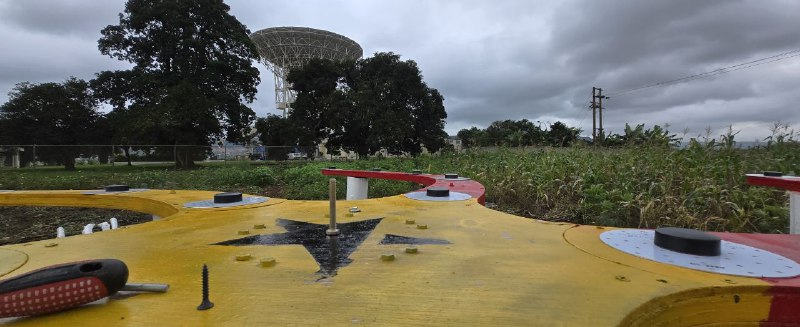
\includegraphics[width=\linewidth]{fig/antenna_9_dish.jpg}
\begin{columns}
 \begin{column}{0.5\linewidth}
  \begin{enumerate}
    \item Identify an antenna arm aligned with a distant landmark visible on satellite imagery
    \item Record GPS coordinates of telescope and landmark
  \end{enumerate}
 \end{column}
 \begin{column}{0.5\linewidth}
  \begin{enumerate}
    \item Compute forward azimuth (bearing)
    \item Constrain that antenna's bearing in the least-squares minimization
  \end{enumerate}
 \end{column}
\end{columns}
\end{frame}

% --- Algorithm ---

\begin{frame}{Optimization Algorithm}
\begin{itemize}
  \item Start with \textbf{initial estimates} $\{x_i, y_i\}$ from the telescope's nominal design (API or JSON config)
  \item Compute simulated measurements:
  \begin{equation*}
    r_i^s = \sqrt{x_i^2 + y_i^2}, \qquad
    \delta_{ij}^s = \sqrt{(x_i - x_j)^2 + (y_i - y_j)^2}
  \end{equation*}
  \item Minimize $L(x,y)$ using \textbf{Trust-Region Reflective} (TRF) least squares (\texttt{scipy.optimize.least\_squares}), bounded to $\pm4.2$~m around each initial coordinate
  \item Compute residuals: $\epsilon_i = r_i - r_i^s$, $\epsilon_{ij} = \delta_{ij} - \delta_{ij}^s$
  \item Flag outliers where $|\epsilon| > \tau$, re-measure, and repeat
  \item Converges when all residuals are acceptable
\end{itemize}
\end{frame}

% --- Flowchart ---

\begin{frame}{Iterative Calibration Process}
\vspace{-8pt}
\begin{center}
\adjustbox{max width=0.5\linewidth}{%
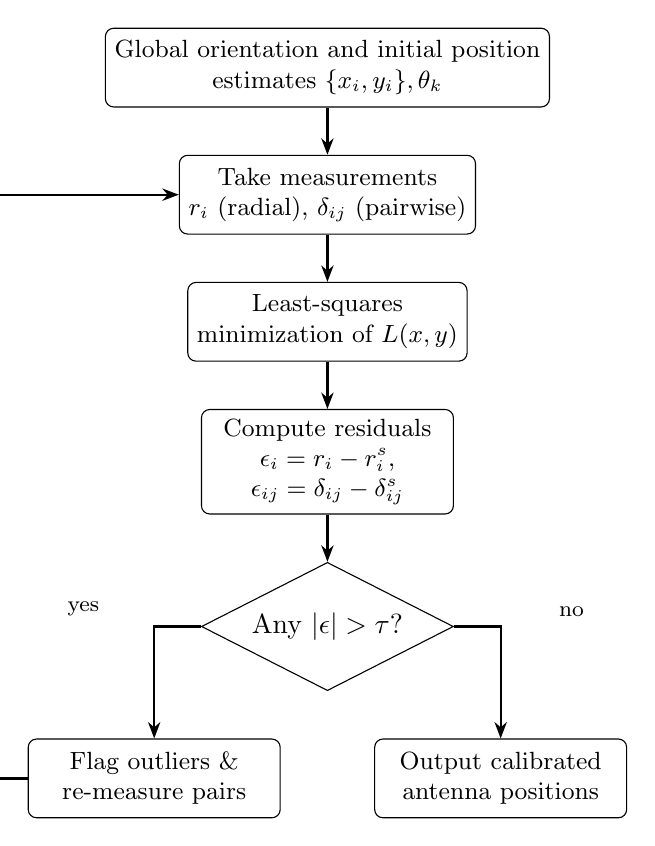
\begin{tikzpicture}[
    node distance=6mm and 4mm,
    box/.style={rectangle, draw, rounded corners=3pt, minimum width=32mm, minimum height=10mm, align=center, font=\small},
    decision/.style={diamond, draw, aspect=1.5, minimum width=32mm, minimum height=10mm, align=center, inner sep=0pt},
    arrow/.style={-{Stealth[scale=0.9]}, thick},
]

\node[box] (start)                    {Global orientation and initial position\\estimates $\{x_i, y_i\}, \theta_k$};
\node[box] (measure) [below=of start] {Take measurements\\$r_i$ (radial), $\delta_{ij}$ (pairwise)};
\node[box] (optimize) [below=of measure] {Least-squares\\minimization of $L(x,y)$};
\node[box] (residuals) [below=of optimize] {Compute residuals\\$\epsilon_i = r_i - r_i^s$,\\$\epsilon_{ij} = \delta_{ij} - \delta_{ij}^s$};
\node[decision] (check) [below=of residuals] {Any $|\epsilon| > \tau$?};
\node[box] (flag) [below=of check, xshift=-22mm] {Flag outliers \&\\re-measure pairs};
\node[box] (done) [below=of check, xshift=22mm]  {Output calibrated\\antenna positions};

\draw[arrow] (start)    -- (measure);
\draw[arrow] (measure)  -- (optimize);
\draw[arrow] (optimize) -- (residuals);
\draw[arrow] (residuals) -- (check);

\draw[arrow] (check) -| node[above, xshift=-9mm, font=\footnotesize] {yes} (flag);
\draw[arrow] (check) -| node[above, xshift=9mm, font=\footnotesize]  {no}  (done);

\draw[arrow, overlay] (flag.west) -- ++(-5mm,0) |- (measure.west);

\end{tikzpicture}%
}
\end{center}
\end{frame}

% --- Symmetries ---

\begin{frame}{Symmetries of the Distance Data}
Distances alone do not fully determine $\{x_i, y_i\}$. Three symmetries leave $r_i$ and $\delta_{ij}$ unchanged:

\vspace{4pt}
\begin{center}
\begin{tabular}{lll}
\hline
Symmetry & Type & Resolved by \\
\hline
Translation & continuous (2 DOF) & phase centre fixed at $(0,0)$ \\
Rotation & continuous (1 DOF) & bearing constraint $\theta_k$ \\
Reflection & discrete ($\mathbb{Z}_2$) & \textbf{not yet resolved} \\
\hline
\end{tabular}
\end{center}

\vspace{8pt}
\textbf{The problem:} a mirror image of the array, reflected across the line at bearing $\theta_k$, preserves every $r_i$, $\delta_{ij}$, \emph{and} $\theta_k$. The true configuration and its reflection are degenerate minima of $L(x,y)$ --- indistinguishable from the residuals alone.
\end{frame}

\begin{frame}{Breaking the Reflection Degeneracy: Chirality}
\begin{itemize}
  \item Pick a second antenna $c$, not collinear with reference antenna $k$ (ideally on a different spiral arm)
  \item From the \emph{initial guess}, compute the cross product and its sign:
  \[
    C = \mathbf{p}_k \times \mathbf{p}_c = x_k y_c - y_k x_c, \qquad s = \operatorname{sign}(C)
  \]
  \item Penalise the optimizer if it flips that sign:
  \[
    L_\chi = \left[ \min\!\left(0,\; s \cdot \frac{x_k y_c - y_k x_c}{r_k r_c}\right) \right]^2
  \]
  \item Normalised by $r_k r_c$ so the penalty is dimensionless ($\approx \sin\theta$); weight $\gamma \approx 10^6$ makes it an effective hard constraint
  \item Zero cost when chirality already matches the initial guess --- only acts if the optimizer tries to cross into the mirror solution
  \item CLI: \texttt{--chirality-index}~$c$ (requires \texttt{--rot-index})
  \item In IRLS mode, $L_\chi$ keeps weight 1 always --- never relaxed by robust down-weighting
\end{itemize}
\end{frame}

% --- Final positions ---

\begin{frame}{Calibrated Positions}
 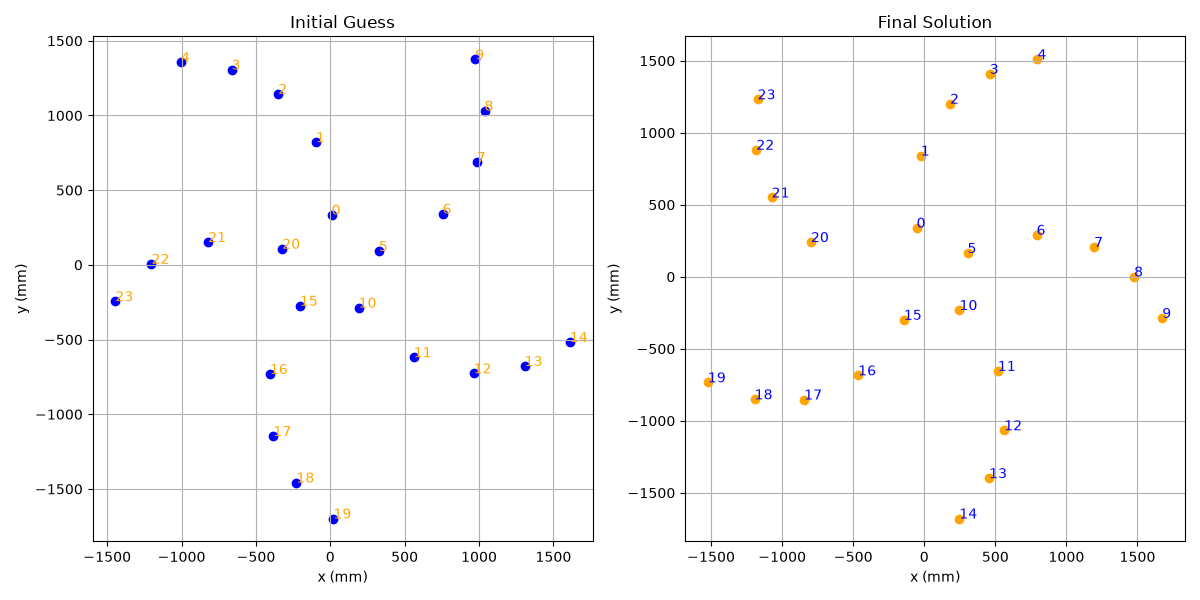
\includegraphics[width=\linewidth]{fig/final_positions.png}
 \vspace{4pt}
 {\small Initial position estimates (blue) and final calibrated positions (orange). The constructed array has clockwise-oriented spiral arms --- opposite to the initial assumption. The chirality constraint is what lets the optimizer find \emph{this} configuration rather than its mirror image.}
\end{frame}

% --- CLI usage ---

\begin{frame}[fragile]{The \texttt{tart-position-cal} Package}
Open-source Python package (GPL-3.0), CLI + programmatic API, installable via \texttt{pip}~\cite{moltento2026tartpositioncal}.

\vspace{6pt}
\begin{lstlisting}[basicstyle=\ttfamily\small, breaklines=true]
tart-position-cal \
    --measurements antenna_measurements.ods \
    --positions antenna_positions.json \
    --output calibrated_antenna_positions.json \
    --rot-index 3 --rot-degrees 18.1125 \
    --chirality-index 10 \
    --irls
\end{lstlisting}

\vspace{4pt}
\begin{itemize}
  \item \texttt{--rot-index}/\texttt{--rot-degrees}: fix global rotation
  \item \texttt{--chirality-index}: fix reflection (handedness)
  \item \texttt{--irls}: robust calibration (next section)
  \item \texttt{compute\_bearing()}: solves the inverse geodesic problem (WGS84, via PROJ) to get \texttt{--rot-degrees} from two lat/lon pairs
\end{itemize}
\end{frame}

% --- UNAM Deployment ---

\begin{frame}{Results: UNAM Deployment}
\vspace{-4pt}
\begin{itemize}
  \item TART telescope at University of Namibia (Windhoek): $(-22.6121^\circ, 17.0568^\circ)$
  \item 24 antennas on 5 spiral arms, max radius $\approx 1.7$~m
\end{itemize}
\vspace{4pt}
\textbf{Initial conditions:}
\begin{itemize}
  \item Initial cost $L(x,y) = 3.5 \times 10^7$ --- substantial disagreement with measurements
\end{itemize}
\vspace{4pt}
\textbf{Global orientation:}
\begin{itemize}
  \item Reference: antenna~3 aligned with distant hill at $(-22.553822^\circ, 17.077290^\circ)$
  \item Computed bearing: $\beta = 18.1125^\circ$; chirality fixed via antenna~10
\end{itemize}
\vspace{4pt}
\textbf{Calibration outcome:}
\begin{itemize}
  \item TRF converged in 20 iterations
  \item Final cost: $L(x,y) = 4.35 \times 10^2$
  \item 90th percentile of absolute residuals: \textbf{1.65~mm} ($\approx 0.009\lambda$ at L1)
\end{itemize}
\end{frame}

% --- UNAM differences ---


% --- Position table ---

\begin{frame}{UNAM Calibrated Antenna Positions}
\vspace{-8pt}
{\small Coordinates in meters relative to phase centre $[0,0]$.}
\begin{center}
\begin{tabular}{|r|r|r||r|r|r|}
\hline
Ant. & $x$ (m) & $y$ (m) & Ant. & $x$ (m) & $y$ (m) \\
\hline
 0 & $-0.054$ &  $0.341$ & 12 &  $0.562$ & $-1.066$ \\
 1 & $-0.025$ &  $0.841$ & 13 &  $0.456$ & $-1.398$ \\
 2 &  $0.181$ &  $1.202$ & 14 &  $0.246$ & $-1.679$ \\
 3 &  $0.461$ &  $1.409$ & 15 & $-0.144$ & $-0.299$ \\
 4 &  $0.796$ &  $1.510$ & 16 & $-0.465$ & $-0.685$ \\
 5 &  $0.304$ &  $0.164$ & 17 & $-0.845$ & $-0.853$ \\
 6 &  $0.790$ &  $0.292$ & 18 & $-1.194$ & $-0.851$ \\
 7 &  $1.195$ &  $0.207$ & 19 & $-1.523$ & $-0.733$ \\
 8 &  $1.476$ &  $0.002$ & 20 & $-0.797$ &  $0.241$ \\
 9 &  $1.674$ & $-0.287$ & 21 & $-1.074$ &  $0.550$ \\
10 &  $0.248$ & $-0.231$ & 22 & $-1.182$ &  $0.882$ \\
11 &  $0.517$ & $-0.654$ & 23 & $-1.173$ &  $1.232$ \\
\hline
\end{tabular}
\end{center}
\end{frame}

% --- Residuals ---

\begin{frame}{Residual Analysis}
\begin{columns}
 \begin{column}{0.5\linewidth}
  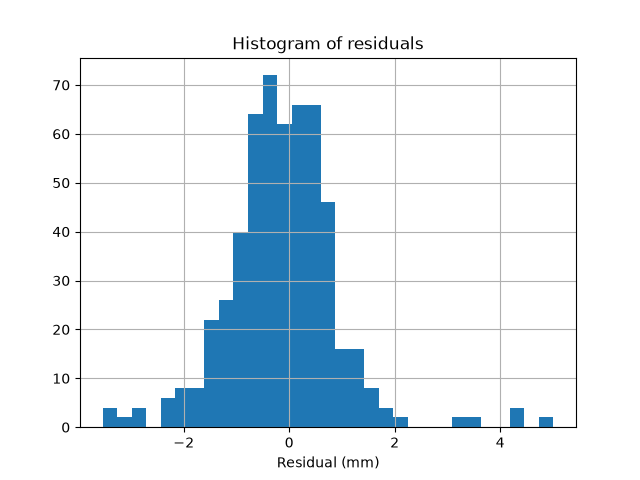
\includegraphics[width=\linewidth]{fig/residual_histogram.png}
  \vspace{4pt}
  {\small Distribution is symmetric around zero, narrow spread.}
 \end{column}
 \begin{column}{0.5\linewidth}
  \begin{itemize}
    \item Residuals = difference between measured and simulated distances after calibration
    \item Median absolute deviation: \textbf{0.63~mm}
    \item Standard deviation: 1.11~mm
    \item 50th / 90th percentile $|$res$|$: 0.59 / \textbf{1.65~mm}
    \item Large residuals flagged for re-measurement in the next iteration
  \end{itemize}
 \end{column}
\end{columns}
\end{frame}

% --- Large residuals ---

\begin{frame}{UNAM: Largest Residuals}
\vspace{-8pt}
{\small Residuals exceeding the 90th percentile (1.65~mm). Negative = measured distance was smaller than calibrated distance.}
\begin{center}
\begin{tabular}{rrr||rrr}
\hline
$i$ & $j$ & Res. (mm) & $i$ & $j$ & Res. (mm) \\
\hline
 9 & 19 & 5.0  &  8 & 17 & $-2.8$ \\
16 & 17 & 4.5  &  0 & 12 & $-2.5$ \\
 2 &  9 & 4.1  &  2 &  5 & $-2.5$ \\
 2 & 13 & $-4.0$ &  4 & 14 & $-2.5$ \\
 3 &  7 & $-3.5$ &  0 & 14 & $-2.4$ \\
 1 & 14 & $-3.5$ &  3 & 12 & $-2.3$ \\
 4 & 17 & 3.4  &    &    &       \\
12 & 22 & 3.1  &    &    &       \\
 4 & 19 & $-3.1$ &    &    &       \\
\hline
\end{tabular}
\end{center}
\vspace{4pt}
{\small These outliers would be re-measured in the next iteration --- or down-weighted automatically by IRLS.}
\end{frame}

% --- IRLS ---

\begin{frame}{Robust Calibration: IRLS}
\begin{columns}
 \begin{column}{0.5\linewidth}
  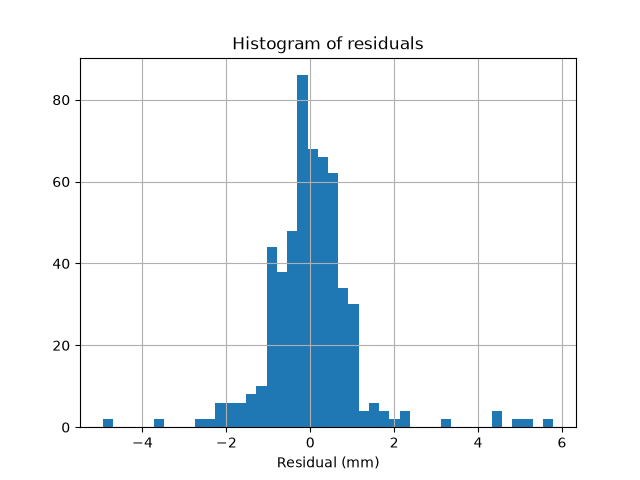
\includegraphics[width=\linewidth]{fig/irls_residual_histogram.png}
  \vspace{4pt}
  {\small IRLS with Tukey weights: 90th percentile improves to \textbf{1.44~mm}.}
 \end{column}
 \begin{column}{0.5\linewidth}
  \begin{itemize}
    \item \texttt{--irls}: re-solves a weighted least-squares problem, recomputing weights each outer iteration to down-weight outliers
    \item \textbf{Tukey} bisquare (default): zeroes out clear outliers
    \item \textbf{Huber}: caps outlier influence with a saturating penalty
    \item Converged in 4 outer iterations for UNAM
    \item MAD: 0.63 $\to$ 0.49~mm; 90th pct: 1.65 $\to$ 1.44~mm
    \item Unweighted objective \emph{rises} ($4.35{\times}10^2 \to 5.40{\times}10^2$) since the down-weighted outliers dominated it
  \end{itemize}
 \end{column}
\end{columns}
\end{frame}

% --- Conclusions ---

\begin{frame}{Conclusions}
\begin{itemize}
  \item Practical, accurate antenna position calibration using only a tape measure and one geographic bearing
  \item Suitable for workshop-based telescope deployments
  \item UNAM: MAD 0.63~mm ($\approx 0.003\lambda$), 90th pct 1.65~mm ($\approx 0.009\lambda$) at L1 --- well within imaging requirements
  \item Outlier flagging \& re-measurement (or IRLS) makes the method robust to inevitable survey errors
  \item Calibrated positions upload directly to the telescope API, ready for imaging
\end{itemize}
\end{frame}

% --- Future Work ---

\begin{frame}{Future Work}
\vspace{-4pt}
\textbf{GNSS-based Calibration:}
\begin{itemize}
  \item TART shares L1 band (1.575~GHz) with GNSS signals
  \item Raw telescope data contain embedded GNSS satellite signals
  \item Software-defined radio post-processing could yield direct TDOA measurements
  \item Potential for fully automated, absolute position calibration without manual surveying
  \item Challenge: low SNR in broad-beam antennas, short baselines ($<$\,2~m) $\to$ nanosecond TDOA
\end{itemize}
\end{frame}

\begin{frame}[allowframebreaks]{References}
\bibliographystyle{plainnat}
\bibliography{position-cal}
\end{frame}

\end{document}
